\newpage

\section{Database} 

	\subsection{Requirements}
	
		\normalsize
		{		
			\begin{enumerate}[itemsep=1pt,parsep=1pt]
				\item Storage of rules
				\item Common non ambiguous names for rules
				\item Organisational Units and Clients
				\item Globally unique identifiers (GUID) for computer objects. 
			\end{enumerate} 		
		}
	
	\subsection{Design}	

		\normalsize
		{
			The design of the database was minimalist given the requirements.
			Fig. \ref{fig:dbdesignoverview} presents the relational design and
			abstraction of the domain concepts.  As seen in presentation admin 
			interface these entities are represented by design patterns.
			The main requirements are satisfied, ``policy'' table for the storage of rules,
			and the representation of clients and organisational units. 	
			\newline			
		}
	
		\begin{figurehere}
			\begin{center}
			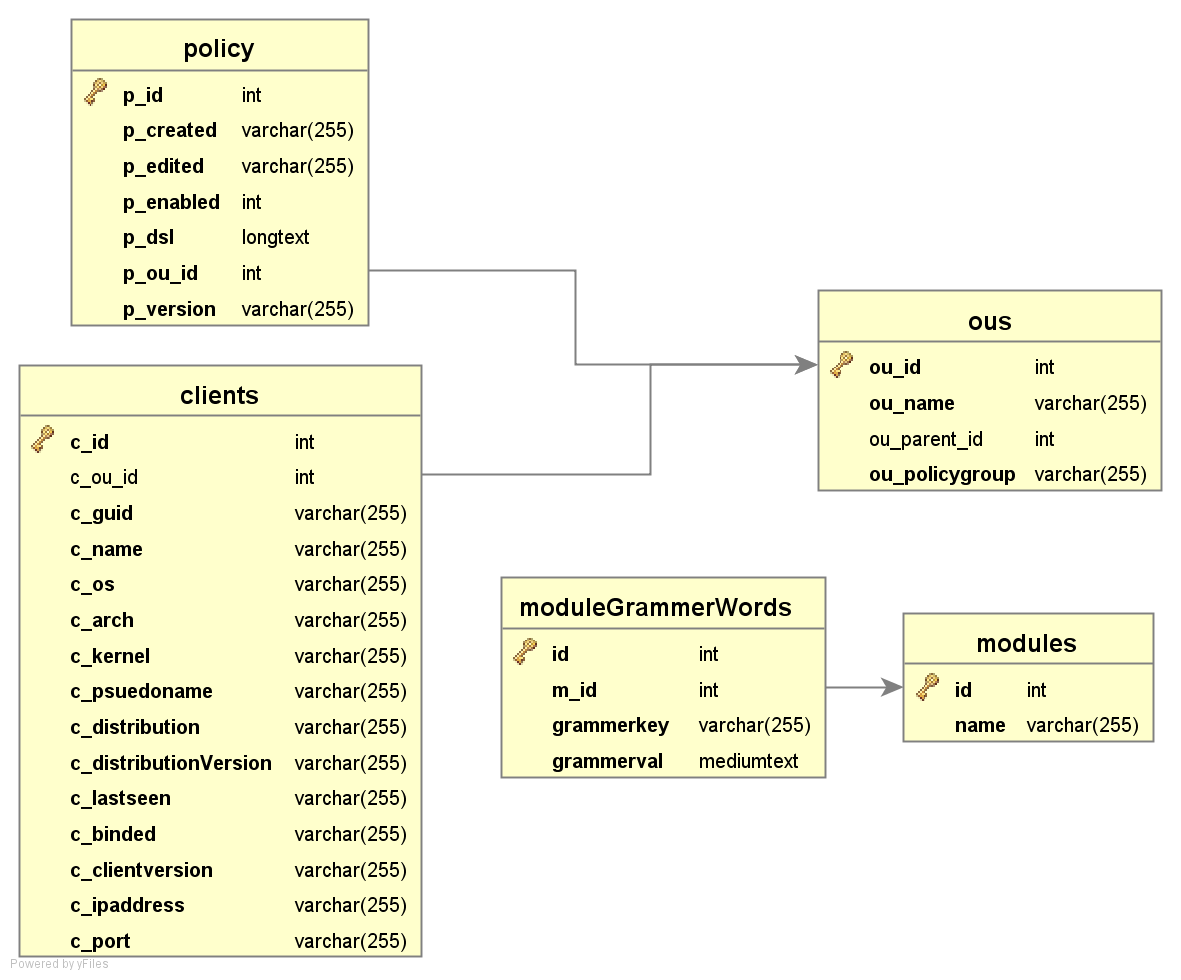
\includegraphics[scale=0.35]{pages/chapter3/figures/db.png}
			\end{center}
			\caption{Database Design Overview}
			\label{fig:dbdesignoverview}
		\end{figurehere}	
	
	\subsection{Analysis \& Improvements}
	
		\normalsize
		{
			Without an analysis of component developer requirements and future development, it's hard to say what improvement would be made to the database design.
			An obvious choice we be the adjustments of the types.  There is extensive used of varchar, however as the data
			is used primarily as strings within the application for display purposes, this may not be necessary.
		}
	
